\documentclass[a4paper]{article}

\usepackage{tikz}
\usetikzlibrary{arrows}

\topmargin -.5in
\textheight 9in
\oddsidemargin -.25in
\evensidemargin -.25in
\textwidth 7in

\begin{document}
	\author{Brandon Thompson 5517}
	\title{Homework 1: EEL 4768.04 Due 9/13/19}
	\maketitle

	\medskip

	\begin{enumerate}
		\item
		What is the largest unsigned 32-bit binary number?\\\\
		The largest possible unsigned binary number is given as:
		\begin{equation}
			2^n-1 \textrm{,\ where $n$ is the number of bits}
		\end{equation}
		Thus the largest 32-bit unsigned binary number is $2^{32}-1 = 18,446,744,073,709,551,615$
		\\ or $1.844674407 \times 10^{19}$.
		\item
		Draw a number line analogous to Figure 1.11 for 3-bit unsigned, two's complement
		and sign/magnitude numbers.\\
		\begin{figure}[h]
			\centering
			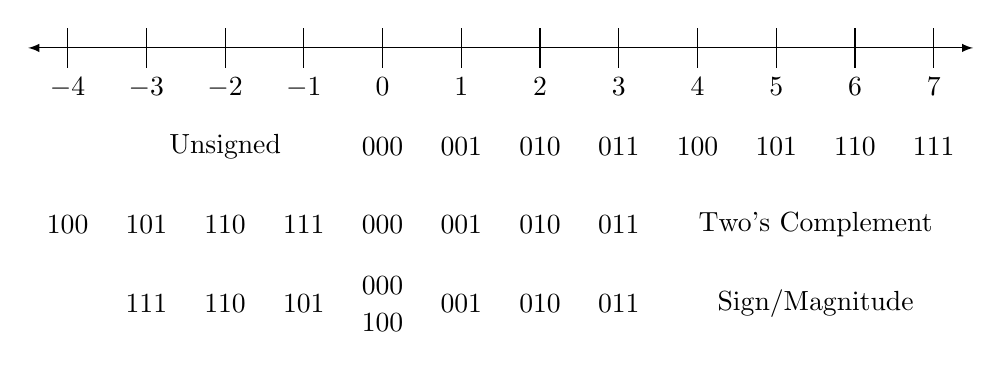
\begin{tikzpicture}
				\draw[latex-latex] (-4.5,0) -- (7.5,0);
				\foreach \x in {-4, -3, ..., 7}
				{
					\draw (\x,0.25) -- (\x, -0.25) node[below] {$\x$};
				}
				\foreach \x [count = \xi] in {000,001,010,011,100,101,110,111}
				{
					\node at (\xi-1,-1.25) {\x};
				}
				\node at (-2,-1.25) {Unsigned};
				\foreach \x [count = \xi] in {100,101,110,111,000,001,010,011}
				{
					\node at (\xi-5,-2.25) {\x};
				}
				\node at (5.5,-2.25) {Two's Complement};
				\foreach \x [count = \xi] in {111,110,101,,001,010,011}
				{
					\node at (\xi-4,-3.25) {\x};
				}
				\node[below] at (0,-3.25) {100};
				\node[above] at (0,-3.25) {000};
				\node at (5.5,-3.25) {Sign/Magnitude};
			\end{tikzpicture}
		\end{figure}	
		\item
		The MIPS architecture has a register set that consists of 32-bit registers. 
		Is it possible to design a computer architecture without a register set? 
		If so, briefly describe the architecture, including the instruction set. 
		What are advantages and disadvantages of this architecture over the MIPS architecture?\\


		Yes, it is possible to have a computer architecture without a register set. Instead
		the architecture would use memory in place of the register set. Instructions would
		be required to access the memory:\\
		\texttt{add 0x01, 0x02, 0x03}\\
		This would add the values of the memory location \texttt{0x02} and \texttt{0x03} and
		store the result in \texttt{0x01}.\\

		Advantages of this architecture is that there are fewer instructions because load and store
		operations are no longer needed. Disadvantages are that every operation would require
		a memory access. Meaning the processor would have to be slowed down or the memory
		smaller. Instruction size would have to be larger to access all of the memory or
		each instruction could only access a small number of memory addresses.
	\end{enumerate}
	
\end{document}
